\documentclass[a4j]{jsarticle}
\usepackage{graphicx}
\usepackage{listings}

\title{2024年度プログラミング\textsc{iii} 演習課題}
\author{学籍番号: 35714121 \\ 氏名: 福富隆大}
\date{2024年10月17日}

\begin{document}
\maketitle

\textbf{1 はじめに} \\

本レポートは演習課題第3回の実行結果をまとめたものである。\\

\textbf{2 課題の実行結果} \\

\textmd{(課題3-1)} \\

課題の実行結果を図1に示す。 \\

\begin{figure}[htbp]
  \centering
  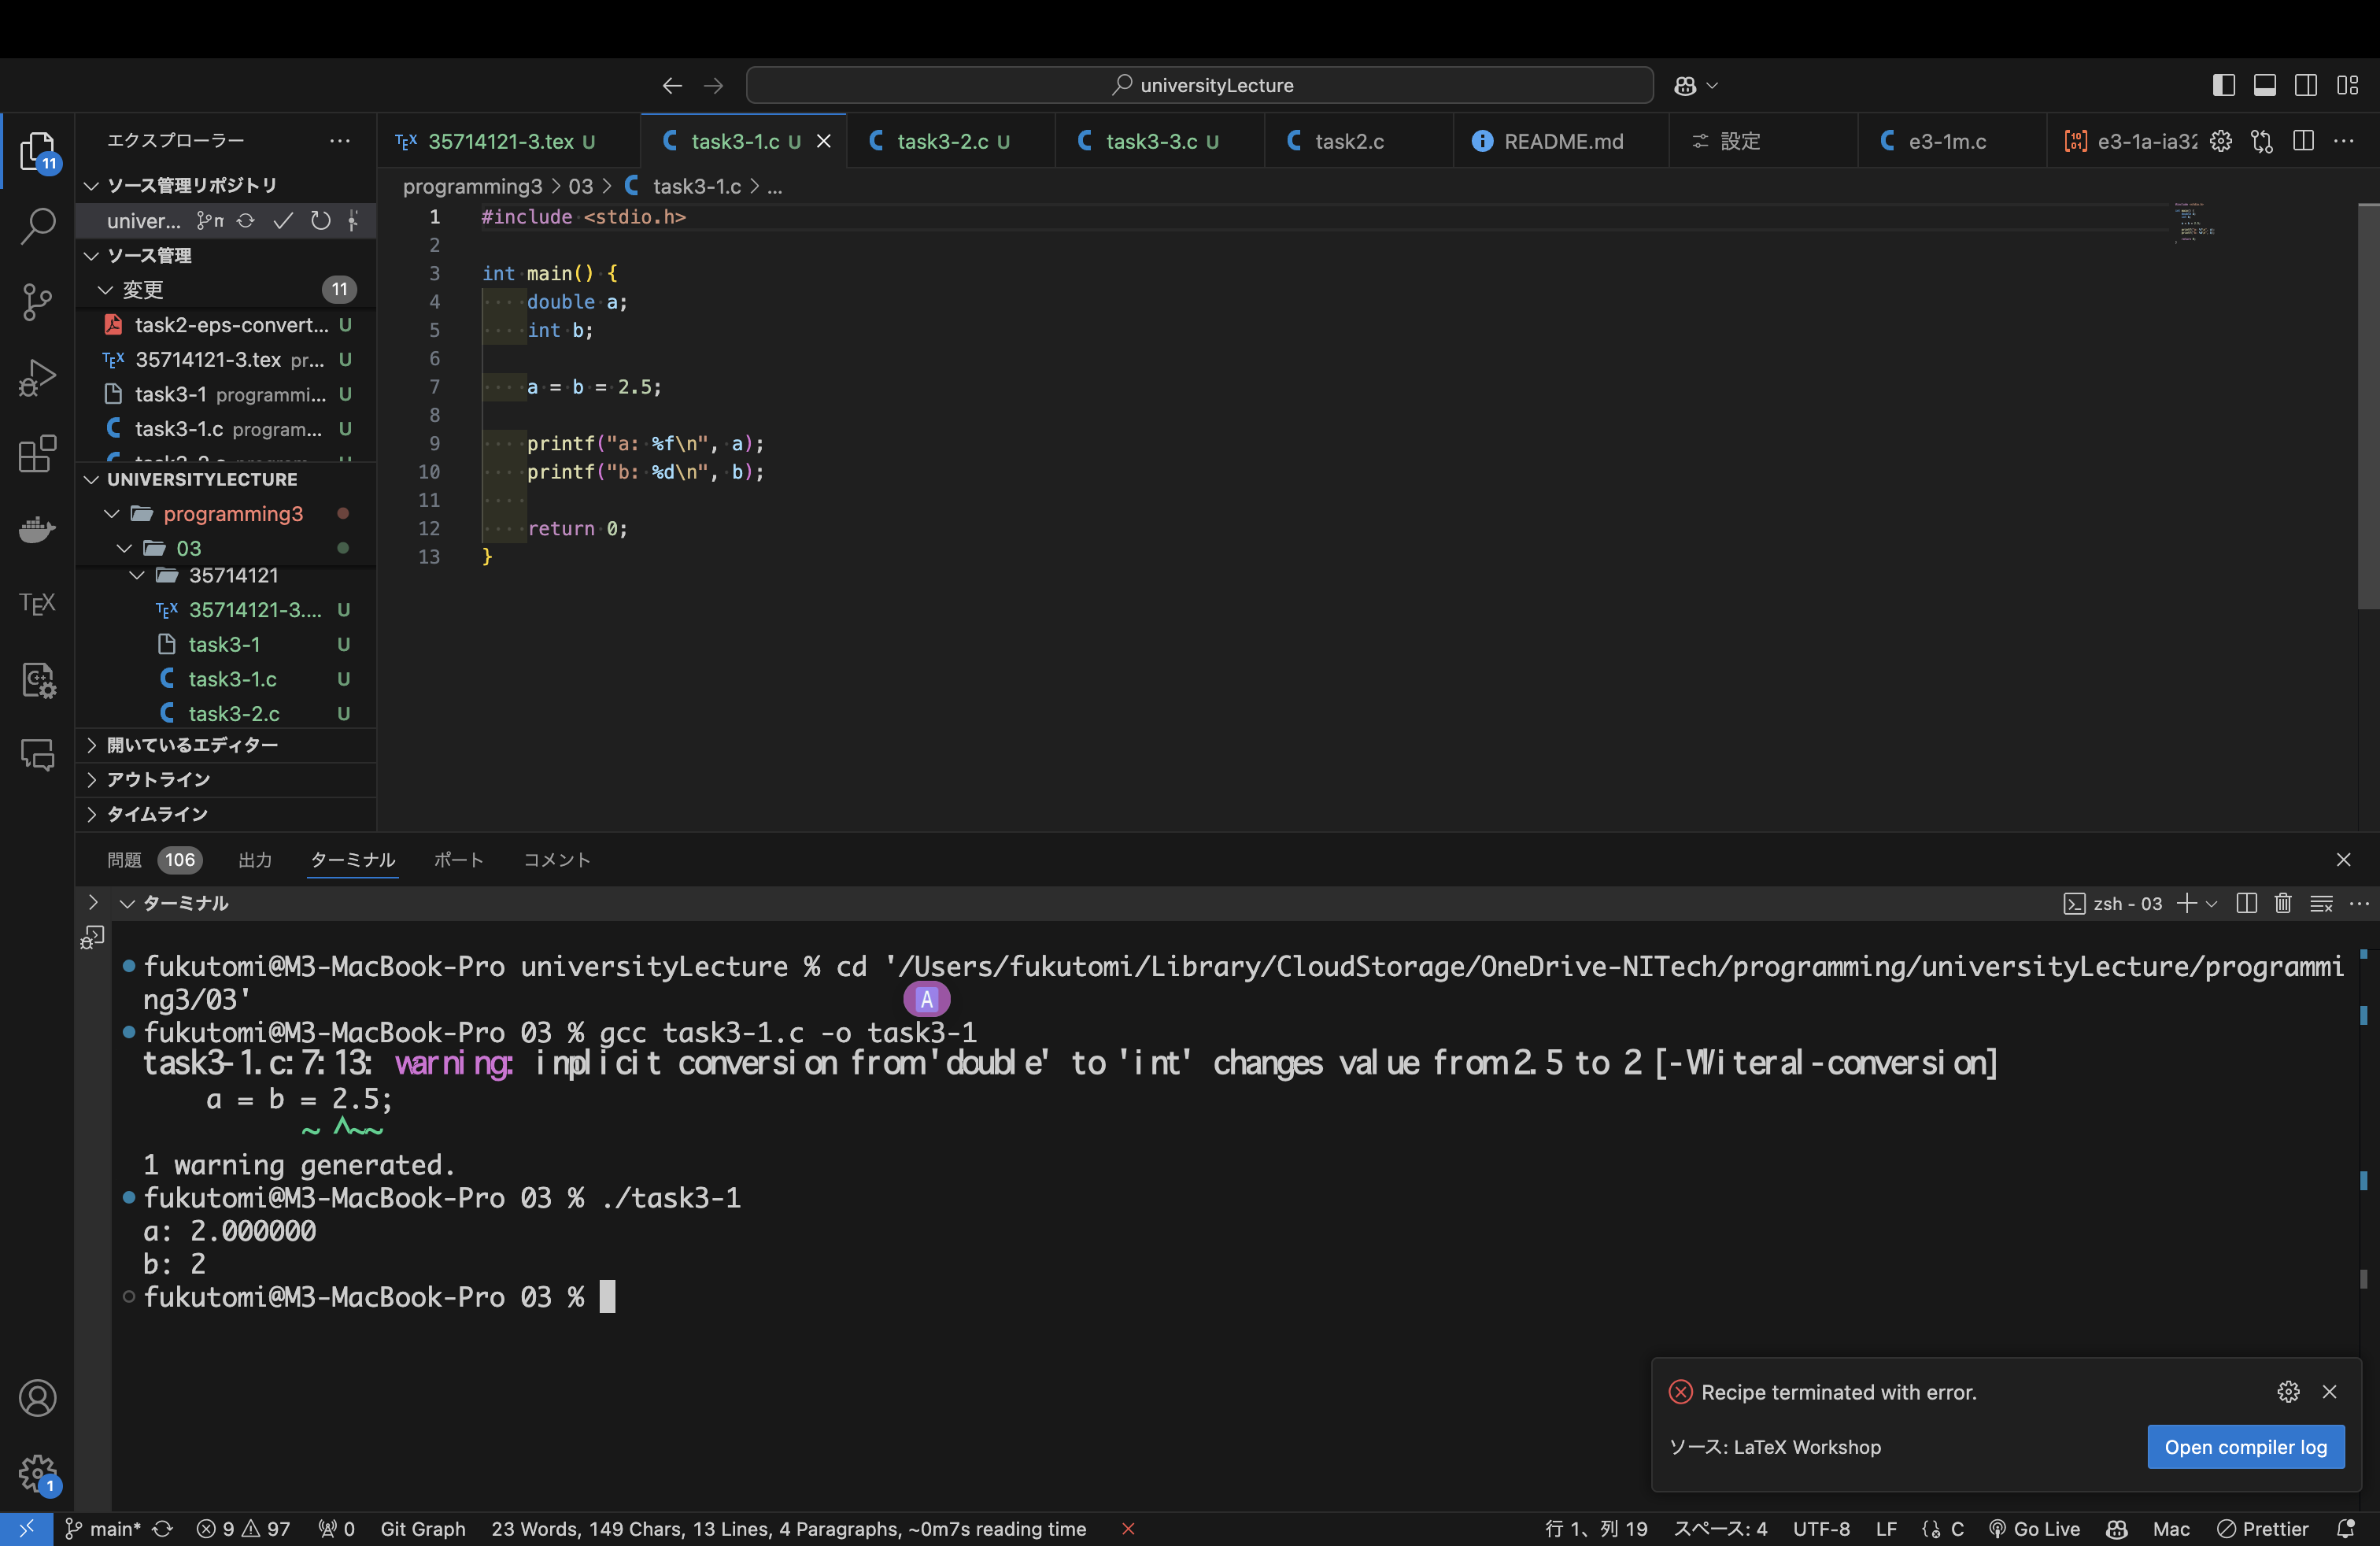
\includegraphics[width=10cm]{task3-1.eps}
  \caption{(ターミナルの部分に実行結果があります)}
  \label{fig:sample}
\end{figure}

\textmd{コードと結果の説明} \\

double型のaとint型のbを宣言し、a = b = 2.5を代入するとa: 2.000000,b: 2となった。  \\
これは、aはdouble型であり、bはint型であるため、bに代入する際に2.5の小数点以下が切り捨てられ、2となり、それがaに代入されたので2.5が2.000000となった。 \\

\textmd{(課題3-2)} \\

課題の実行結果を図2に示す。\\

\begin{figure}[htbp]
  \centering
  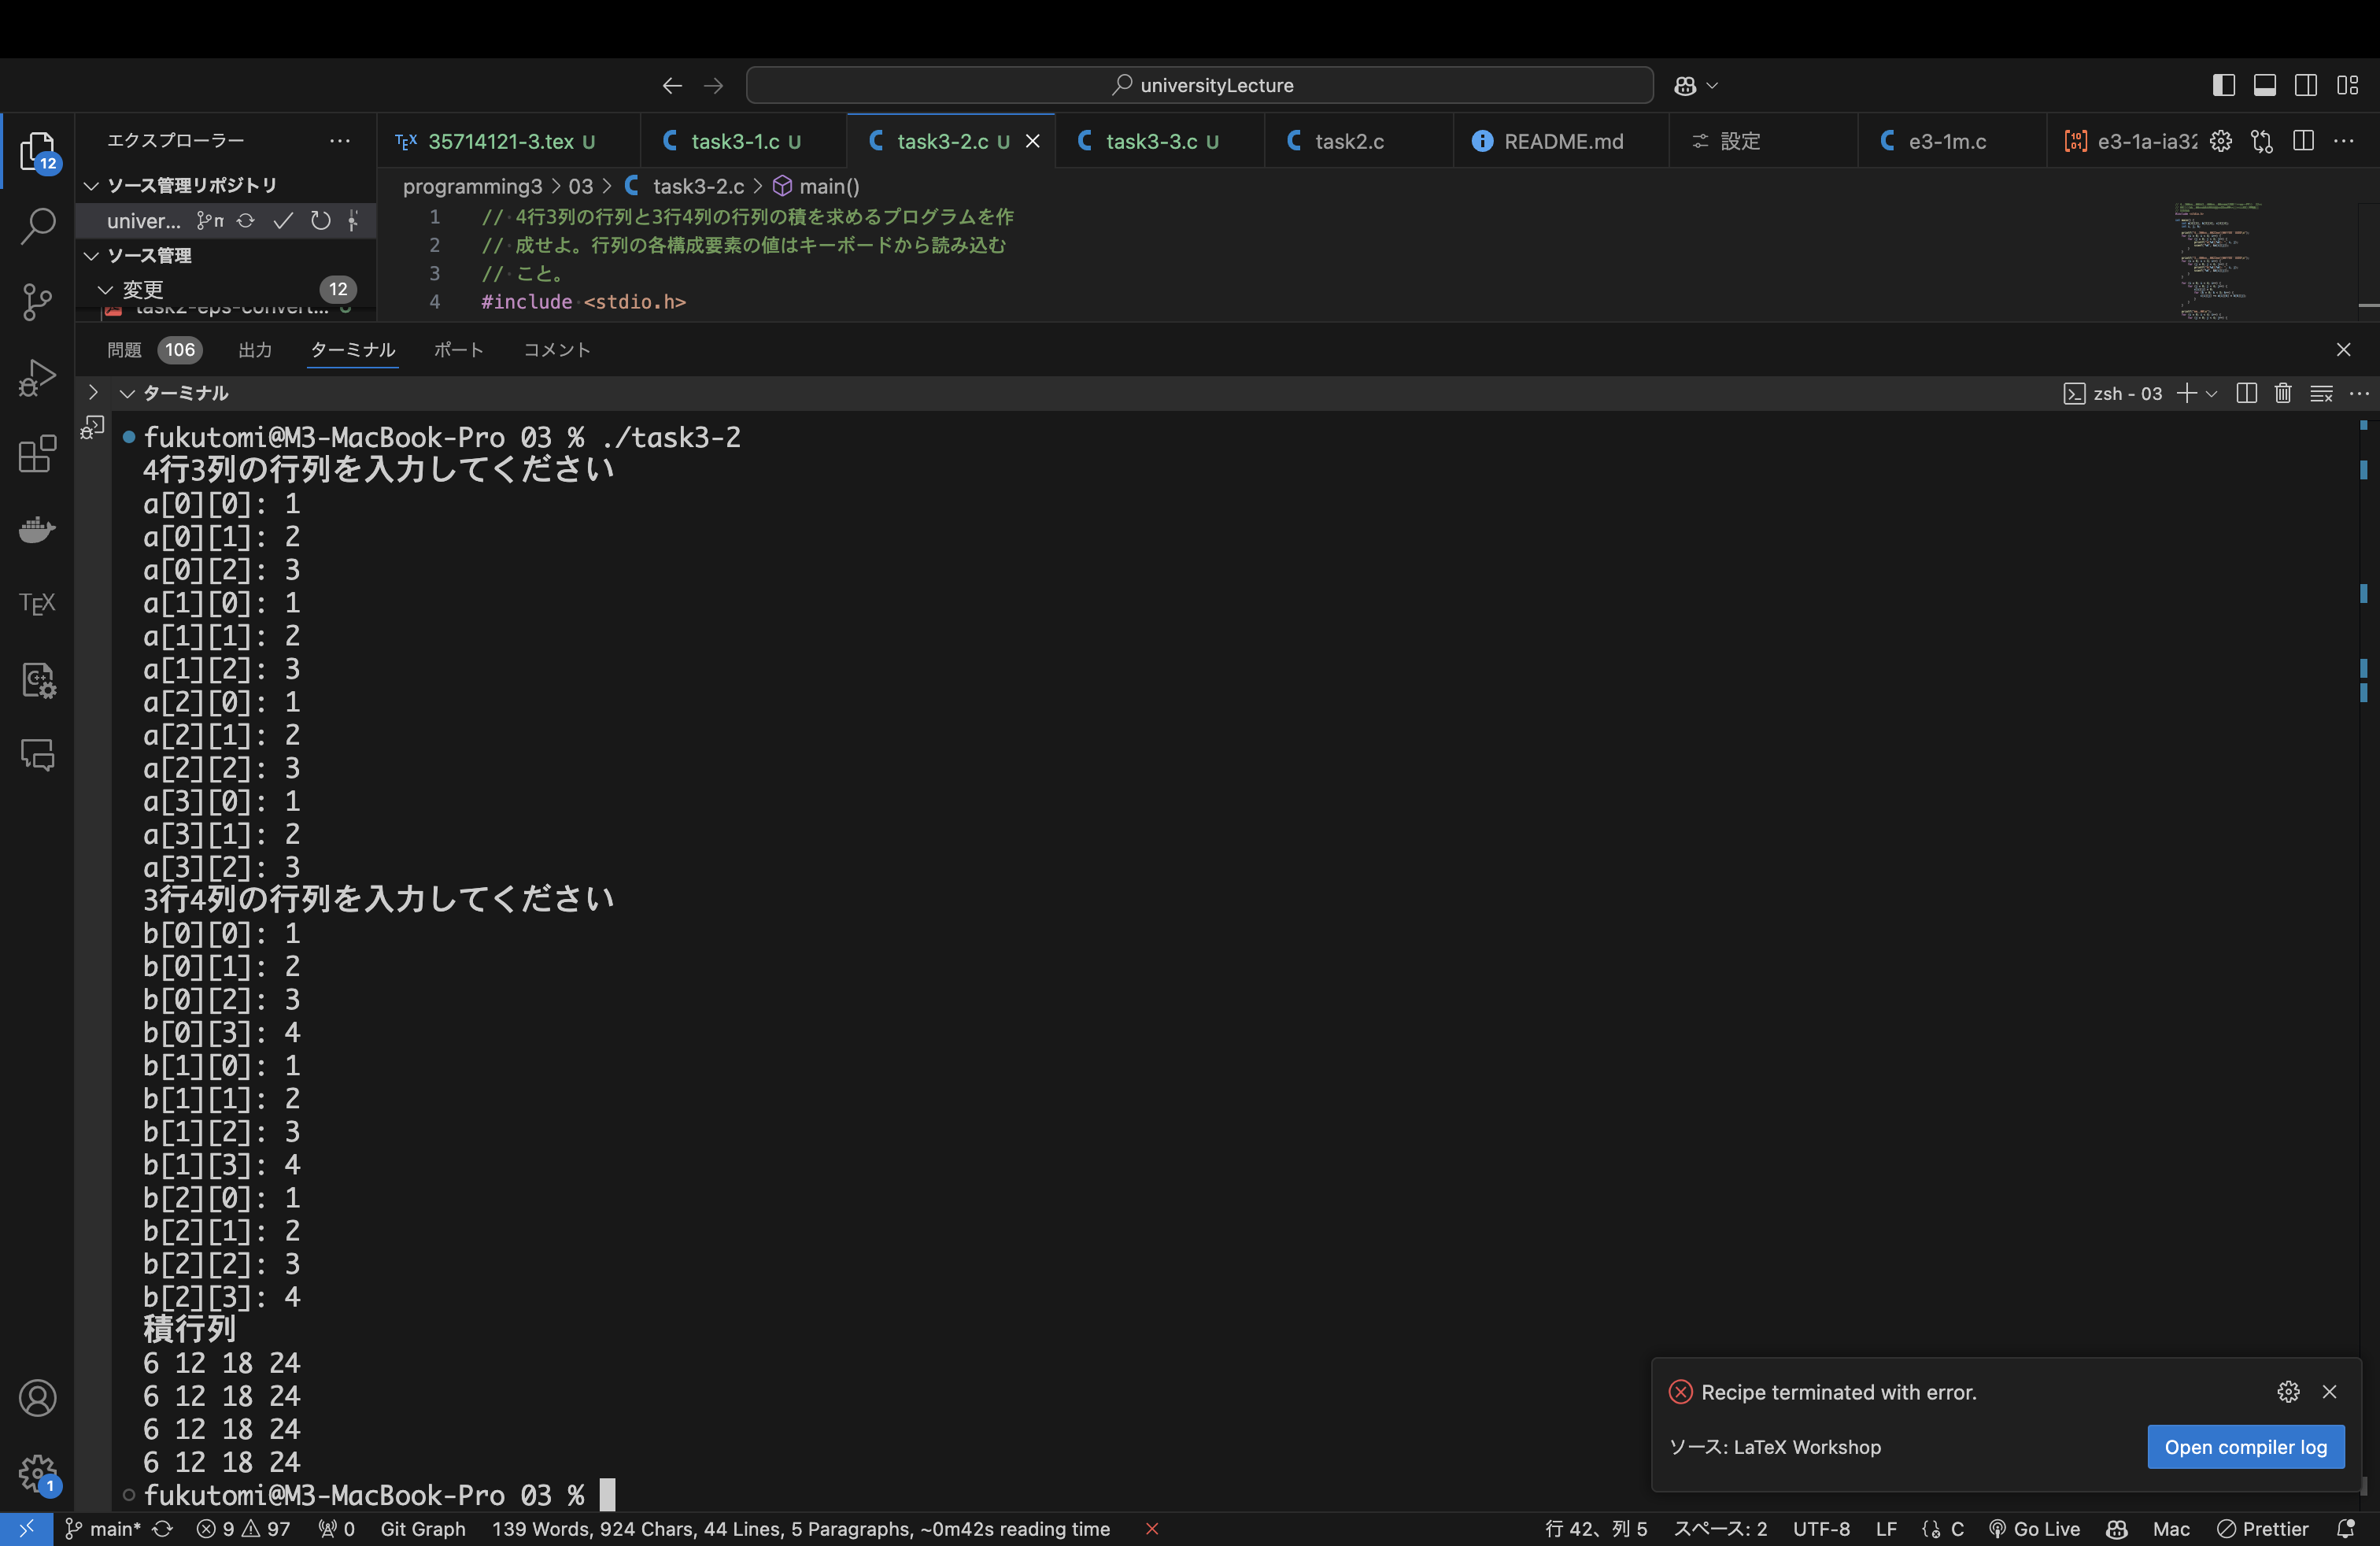
\includegraphics[width=10cm]{task3-2.eps}
  \caption{(ターミナルの部分に実行結果があります)}
  \label{fig:sample}
\end{figure}

\textmd{コードと結果の説明} \\
行列の値を入力してもらう処理をfor分で行い、その後行列の積を計算する処理をfor文で行った。  \\
行列の積を計算する前に、計算結果を入れる配列を0で初期化してそこに足していく形で計算を行った。 \\
その後に、計算結果を出力する処理を行った。  \\

\textmd{(課題3-3)} \\

課題の実行結果を図3に示す。\\

\begin{figure}[htbp]
  \centering
  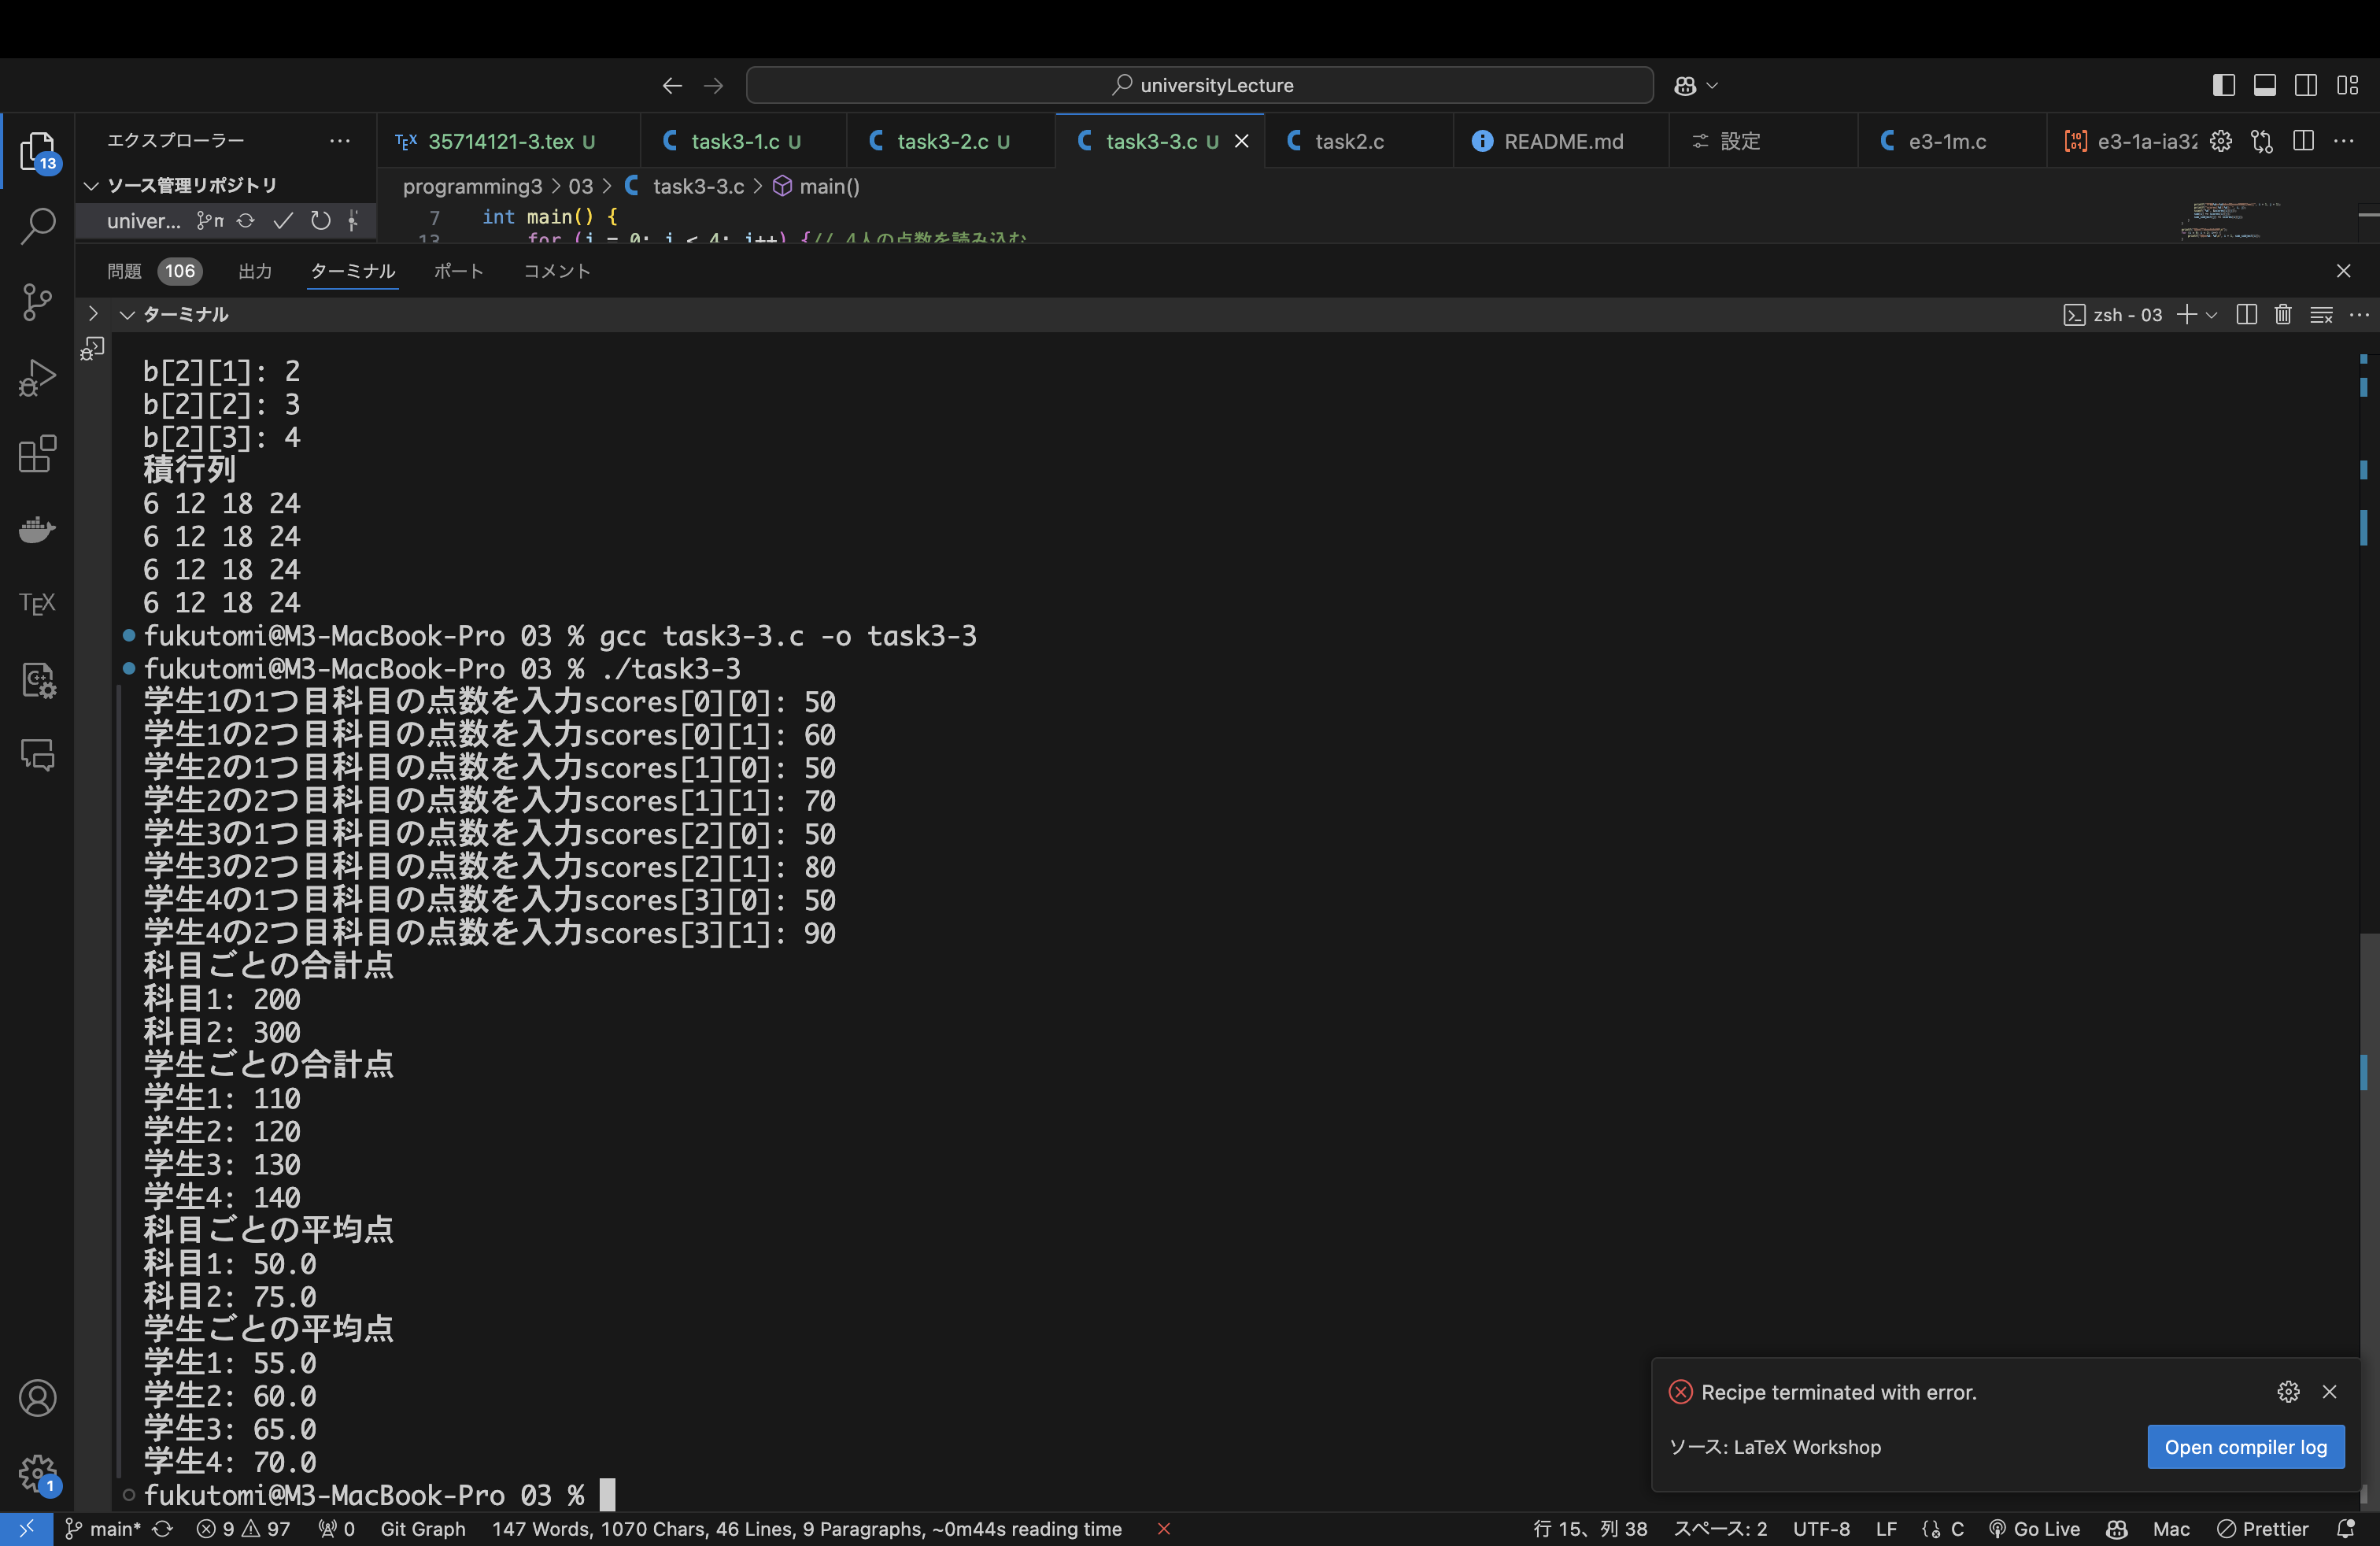
\includegraphics[width=10cm]{task3-3.eps}
  \caption{(ターミナルの部分に実行結果があります)}
  \label{fig:sample}
\end{figure}

\textmd{コードと結果の説明} \\

まず、テスト結果をを入力してもらう処理をfor文で行い、入力の際に点数の合計を格納する用の配列に加算していく処理を行った。 \\
学生や科目の識別がしやすいように、for文で使った変数を用いて学生1、科目1のように表示している。 \\
合計は合計を格納する配列の値をそのまま出力し、平均は合計を人数で割って出力している。  \\
平均は割る処理が入るので少数も表せるようにdouble型にしている。  \\

\end{document}
